% The document class supplies options to control rendering of some standard
% features in the result.  The goal is for uniform style, so some attention 
% to detail is *vital* with all fields.  Each field (i.e., text inside the
% curly braces below, so the MEng text inside {MEng} for instance) should 
% take into account the following:
%
% - author name       should be formatted as "FirstName LastName"
%   (not "Initial LastName" for example),
% - supervisor name   should be formatted as "Title FirstName LastName"
%   (where Title is "Dr." or "Prof." for example),
% - degree programme  should be "BSc", "MEng", "MSci", "MSc" or "PhD",
% - dissertation title should be correctly capitalised (plus you can have
%   an optional sub-title if appropriate, or leave this field blank),
% - dissertation type should be formatted as one of the following:
%   * for the MEng degree programme either "enterprise" or "research" to
%     reflect the stream,
%   * for the MSc  degree programme "$X/Y/Z$" for a project deemed to be
%     X%, Y% and Z% of type I, II and III.
% - year              should be formatted as a 4-digit year of submission
%   (so 2014 rather than the accademic year, say 2013/14 say).

\documentclass[ % the name of the author
                    author={Tom Jager},
                % the name of the supervisor
                supervisor={Dr. Daniel Schien},
                % the degree programme
                    degree={MEng},
                % the dissertation    title (which cannot be blank)
                     title={A Bayesian Inference Engine for UMIS Structured Data},
                % the dissertation subtitle (which can    be blank)
                  subtitle={},
                % the dissertation     type
                      type={research},
                % the year of submission
                      year={2019} ]{dissertation}

\begin{document}

% =============================================================================

% This section simply introduces the structural guidelines.  It can clearly
% be deleted (or commented out) if you use the file as a template for your
% own dissertation: everything following it is in the correct order to use 
% as is.

% =============================================================================

% This macro creates the standard UoB title page by using information drawn
% from the document class (meaning it is vital you select the correct degree 
% title and so on).

\maketitle

% After the title page (which is a special case in that it is not numbered)
% comes the front matter or preliminaries; this macro signals the start of
% such content, meaning the pages are numbered with Roman numerals.

\frontmatter

% This macro creates the standard UoB declaration; on the printed hard-copy,
% this must be physically signed by the author in the space indicated.

\makedecl

% LaTeX automatically generates a table of contents, plus associated lists 
% of figures, tables and algorithms.  The former is a compulsory part of the
% dissertation, but if you do not require the latter they can be suppressed
% by simply commenting out the associated macro.

\tableofcontents
% \listoffigures
% \listoftables
% \listofalgorithms
% \lstlistoflistings

% The following sections are part of the front matter, but are not generated
% automatically by LaTeX; the use of \chapter* means they are not numbered.

% -----------------------------------------------------------------------------

\chapter*{Executive Summary}

{\bf A compulsory section, of at most $1$ page} 
\vspace{1cm} 

\noindent
This section should pr\'{e}cis the project context, aims and objectives,
and main contributions (e.g., deliverables) and achievements; the same 
section may be called an abstract elsewhere.  The goal is to ensure the 
reader is clear about what the topic is, what you have done within this 
topic, {\em and} what your view of the outcome is.

The former aspects should be guided by your specification: essentially 
this section is a (very) short version of what is typically the first 
chapter.  Note that for research-type projects, this {\bf must} include 
a clear research hypothesis.  This will obviously differ significantly
for each project, but an example might be as follows:

\begin{quote}
My research hypothesis is that a suitable genetic algorithm will yield
more accurate results (when applied to the standard ACME data set) than 
the algorithm proposed by Jones and Smith, while also executing in less
time.
\end{quote}

\noindent
The latter aspects should (ideally) be presented as a concise, factual 
bullet point list.  Again the points will differ for each project, but 
an might be as follows:

\begin{quote}
\noindent
\begin{itemize}
\item I spent $120$ hours collecting material on and learning about the 
      Java garbage-collection sub-system. 
\item I wrote a total of $5000$ lines of source code, comprising a Linux 
      device driver for a robot (in C) and a GUI (in Java) that is 
      used to control it.
\item I designed a new algorithm for computing the non-linear mapping 
      from A-space to B-space using a genetic algorithm, see page $17$.
\item I implemented a version of the algorithm proposed by Jones and 
      Smith in [6], see page $12$, corrected a mistake in it, and 
      compared the results with several alternatives.
\end{itemize}
\end{quote}


\chapter*{Supporting Technologies}

{\bf A compulsory section, of at most $1$ page}
\vspace{1cm} 

\noindent
This section should present a detailed summary, in bullet point form, 
of any third-party resources (e.g., hardware and software components) 
used during the project.  Use of such resources is always perfectly 
acceptable: the goal of this section is simply to be clear about how
and where they are used, so that a clear assessment of your work can
result.  The content can focus on the project topic itself (rather,
for example, than including ``I used \mbox{\LaTeX} to prepare my 
dissertation''); an example is as follows:

\begin{quote}
\noindent
\begin{itemize}
\item I used the Java {\tt BigInteger} class to support my implementation 
      of RSA.
\item I used a parts of the OpenCV computer vision library to capture 
      images from a camera, and for various standard operations (e.g., 
      threshold, edge detection).
\item I used an FPGA device supplied by the Department, and altered it 
      to support an open-source UART core obtained from 
      \url{http://opencores.org/}.
\item The web-interface component of my system was implemented by 
      extending the open-source WordPress software available from
      \url{http://wordpress.org/}.
\end{itemize}
\end{quote}

% -----------------------------------------------------------------------------

\chapter*{Notation and Acronyms}

{\bf An optional section, of roughly $1$ or $2$ pages}
\vspace{1cm} 

\noindent
Any well written document will introduce notation and acronyms before
their use, {\em even if} they are standard in some way: this ensures 
any reader can understand the resulting self-contained content.  

Said introduction can exist within the dissertation itself, wherever 
that is appropriate.  For an acronym, this is typically achieved at 
the first point of use via ``Advanced Encryption Standard (AES)'' or 
similar, noting the capitalisation of relevant letters.  However, it 
can be useful to include an additional, dedicated list at the start 
of the dissertation; the advantage of doing so is that you cannot 
mistakenly use an acronym before defining it.  A limited example is 
as follows:

\begin{quote}
\noindent
\begin{tabular}{lcl}
IE                 &:     & Industrial Ecology                                         \\
IOA                &:     & Input Output Assessment
  \\
LCA                &:     & Life Cycle Assessment
  \\
MFA                &:     & Material Flow Assessment
  \\
UMIS               &:     & Unified Materials Information System
  \\
YSTAFDB            &:     & Yale Stocks and Flows Database
  \\
STAFDB             &:      &  Stocks and Flows Database
  \\
\end{tabular}
\end{quote}

% -----------------------------------------------------------------------------

\chapter*{Acknowledgements}

{\bf An optional section, of at most $1$ page}
\vspace{1cm} 

\noindent
It is common practice (although totally optional) to acknowledge any
third-party advice, contribution or influence you have found useful
during your work.  Examples include support from friends or family, 
the input of your Supervisor and/or Advisor, external organisations 
or persons who  have supplied resources of some kind (e.g., funding, 
advice or time), and so on.

% =============================================================================

% After the front matter comes a number of chapters; under each chapter,
% sections, subsections and even subsubsections are permissible.  The
% pages in this part are numbered with Arabic numerals.  Note that:
%
% - A reference point can be marked using \label{XXX}, and then later
%   referred to via \ref{XXX}; for example Chapter\ref{chap:context}.
% - The chapters are presented here in one file; this can become hard
%   to manage.  An alternative is to save the content in seprate files
%   the use \input{XXX} to import it, which acts like the #include
%   directive in C.

\mainmatter

% -----------------------------------------------------------------------------

\chapter{Contextual Background}
\label{chap:context}

\noindent
\section{Industrial Ecology}

Industrial ecology (IE) is an area of research focused around the flow of material, energy and money through a system. It can also be described as socio-economic metabolism (SEM) as it models the production, consumption and storage of resources by society. It primarily focuses on the relationship between human originating sectors (anthroposphere) and the natural ecosystem by modelling industrial infrastructures as their own subsystems that interact with their environment \cite{tibbs1992industrial}. The International Society for Industrial Ecology uses the following definition by White, "the study of the flows of materials and energy in industrial and consumer activities, of the effects of these flows on the environment, and of the influences of economic, political, regulatory and social factors on the flow, use and transformation of resources" \cite{white1994greening}. As such it is a multi-disciplinary field which seeks to account for material and energy data and use it to inform social and economic policy as well as business strategy. The primary motivator for Industrial Ecology is to encourage and ensure sustainable development. By most agreed definitions, this involves ensuring that the economical and societal growth occurs without hampering the ability of development in the future \cite{robert2005sustainable}. Therefore research in Industrial Ecology focuses on decoupling the relationship industrial development has on natural ecosystems. To do this, the entire life cycle of products and materials are analyzed in order to find areas for greater efficiency and reduced reliance on natural resources. Studies in Industrial Ecology can focus on identifying the amount of flow of specific materials from the anthroposphere into the environment \cite{rockstrom2009safe}, to assessing where new stocks of materials are accumulating \cite{müller2014modeling}, or finding energy and material "loops" which can be closed in order to reuse waste material and energy\cite{esty1998industrial}.

\subsection{Industrial Ecology Methodology}
There exist a variety of different methodologies to conduct studies in Industrial Ecology. The data resulting from IE studies therefore is usually in a format only suited for that methodology. The three most prevalent methods are Life Cycle Assessments (LCAs), Input-Output Analysis (IOA) and Material Flow Analysis (MFA) \cite{myers2019unified}.

Life Cycle Assessments follow the environmental impact of a product system throughout its life cycle \cite{ISO14040}. It often involves compiling an inventory analysis where the life cycle is modelled as a system of processes with material and energy flowing between them. Inputs and outputs from each process are specified with special interest paid to flows into and from the environment. This is used to assess the impact of a product and provide information for corporate decision making in order to improve the efficiency of a product. Other motivators are in reducing a product's environmental impact. LCAs have been known to have sector wide impacts through industry collaboration \cite{mattila2012methodological}. Open data formats such as EcoSpold and ILCD as well as shared databases such as Ecoinvent \cite{wernet2016ecoinvent}, make this possible as different industry partners can combine research and also easily recreate results to ensure accuracy. 

Input-Output Analyses takes an economic approach to IE and tracks the flow of money between entities in a geographic region. These can then be used to allocate environmental impact to these entities. As economic data on inter-sector flows are generally more granular than data on the movement of physical material, it can be useful to apply data from IOAs in studies that use other methodologies \cite{chen2016building}.

Material and Energy Flow Analyses maps the presence of a specific material(s) in a system, paying particular attention to where it accumulates in the form of stocks. It does this by modelling a system as a collection of processes and then accounting for flows between and the build up of stocks in them. This is useful for identifying where cycles can be created and enhanced in these systems in order to increase recycling and therefore reduce a system's dependence on its environment \cite{müller2014modeling}. Static MFAs are where the scope of the analyses falls over a single specified timeframe, whilst dynamic MFAs use data about past and present quantities to estimate future impacts. This can highlight which resources may become scarce in the future and provide warnings about future environmental impacts.

\section{Unifying Industrial Ecology}
Whilst some studies have incorporated data from one methodology into another \cite{chen2016building}, there is need to provide a common framework for all varieties of industrial ecological data. In \cite{pauliuk2015general}, Pauliuk et al performed a comprehensive analysis on the myriad of methodologies present in IE. They discovered that each methodology described the system using a shared structure, that of a bipartite directed graph. The shared common property between each system is that material was \textit{transformed} in one process and then \textit{distributed} in a subsequent process. Edges in this bipartite graph denote a flow of material from one a \textit{distribution} node to a \textit{transformation} node or vice versa.

\subsection{STAFDB and UMIS}
Over the past 20 years, the Graedal research group at Yale University have compiled Industrial Ecology data on over 100 materials on a variety of spacial and temporal scales. The data from these studies has been extracted and used to create the Yale Stocks and Flows Database (YSTAFDB) \cite{ystafdb}. Ongoing work by Myers, Hoekman and Petard (to be published), is in developing a community driven database for this data called the Stocks and Flows Database (STAFDB). This is an improvement on YSTAFDB as it is designed to be more user friendly and deals with the problem of divergent disaggregation.

Disaggregation is where a property of data (e.g a process that data is coming from or the material being described) is divided into components. In a broad example, data about cars could be disaggregated into electric and non-electric vehicles or large and small cars. If data from two studies with different techniques of disaggregation (or divergent disaggregation) on the same data were structured into the same system, data could be counted twice when performing analysis \cite{myers2019unified}. To prevent this, process and material data in STAFDB contains a parent field and an \texttt{is\_separator} flag which serves to keep track of methods of disaggregation and prevent double counting.

Myers et al. has created UMIS, the Unified Materials Information System \cite{myers2019unified} as a data format to structure data contained in STAFDB. UMIS structures stocks and flows data that comprise IE studies into a format that is agnostic to IOA, MFA and LCA methodologies as a UMIS diagram. This diagram can displayed visually and is also machine readable which allows for greater automation when dealing with stocks and flows data.

UMIS is a step in shifting industrial ecology towards a more virtual platform where industrial ecological data can be stored in a centralized knowledge base, with an ecosystem of tools and routines to develop models and analyze the data for further studies. This would reduce the time taken to perform further studies, allow of greater collaboration in the field and provide greater transparency on the results of studies \cite{hertwich2018nullius}. An example of such a platform is the Metabolism Of Cities project, a digital research lab created by Paul Hoekman \cite{MetabolismOfCities}. The platform's primary aim is to encourage research and allow collaboration in studying the metabolism of resources and energy surrounding specific regions. It contains a store of publications, IE data and an online material flow analysis tool to allow users to easily conduct MFA studies and interface with a common online database. Work is currently being done to integrate metabolism of cities with STAFDB to allow for future research to be directly inserted into the database. 

\subsubsection{UMIS Terminology}
The components and design of a UMIS diagram are drawn from MFA concepts but can still be reconciled with IOA and LCA data. A definition list for the components of a UMIS diagram can be found in table \ref{umis_terms}.

\begin{table}[ht]
\begin{tabular}{|l|l|}
\hline
{\textbf{UMIS Component}}   & {\textbf{Definition}}                                                                                                                                                                                                                                          \\ \hline
System Boundary        & \begin{tabular}[c]{@{}l@{}}Definition of the boundary of the data. This is defined by the reference\\ space, time frame and material. Provides a limit of what parts of the real\\ world we are interested in and modelling in this system\end{tabular}   \\ \hline
Reference Space        & \begin{tabular}[c]{@{}l@{}}The geographical space within which all processes, stocks and flows\\ internal to the UMIS diagram reside.\end{tabular}                                                                                                        \\ \hline
Reference Material     & \begin{tabular}[c]{@{}l@{}}The material whose stocks and flows are described in the diagram. Can be\\ at a high level of disaggregation (e.g a diagram with a reference material\\ of Steel can contain stocks and flows of Carbon and Iron)\end{tabular} \\ \hline
Reference Time frame   & The time frame over which material is flowing or is stocked.                                                                                                                                                                                              \\ \hline
Process                & An event involving a material                                                                                                                                                                                                                             \\ \hline
Transformation Process & A process where an object is transformed into another object                                                                                                                                                                                              \\ \hline
Distribution Process   & A process where an object is transferred to another process or location                                                                                                                                                                                   \\ \hline
Storage Process        & A process where material is moved into or from storage                                                                                                                                                                                                    \\ \hline
Stock                  & Movement of material between a process and storage                                                                                                                                                                                                        \\ \hline
Flow                   & \begin{tabular}[c]{@{}l@{}}Movement of material between a transformation and distribution process\\ inside the diagram\end{tabular}                                                                                                                       \\ \hline
Cross boundary flow    & \begin{tabular}[c]{@{}l@{}}Movement from material outside the diagram to an internal transformation\\ or distribution process.\end{tabular}                                                                                                               \\ \hline
\end{tabular}
\caption{Components of a UMIS diagram}
\label{umis_terms}
\end{table}

A UMIS diagram can be thought to consist of three layers, a processes and flows layer, a virtual reservoir layer and a metadata layer. The processes and flows layer builds of the work of Pauliuk in \cite{pauliuk2015general}, and structures the system as flows between transformation and distribution processes in the form of a bipartite directed graph. The virtual reservoir lies on top of this graph and contains information relating to stock. When material is moved in or out of storage in a system, it is represented by moving into or out of the virtual reservoir. As processes represent physical locations in a system, stock are only positioned on top of existing processes. The metadata layer is for storing additional information about stocks flows and processes. This is information concerning the reference space or time frame of a component, source of the data, uncertainty around a quantity's value, unit of the value, calculation details e.t.c. A visualization of the key aspects of a UMIS diagram can be seen in figure \ref{fig:umis_aspects}. In order to ensure that UMIS diagrams are able to be computer generated, transformation processes are enforced to have only one outflow to a distribution process. If a system's design indicates a flow from a transformation process to multiple distribution processes, the processes must be further disaggregated to separate them. 

\subsubsection{Divergent Disaggregation}
UMIS also deals with the divergent dissagregation problem present in processes and materials. This is done by assigning every process and material a parent field and an \texttt{is\_separator} flag. The parent field contains the process or materials at the next higher level of aggregation. For example the parent field for a blue car material would be car. As a result the processes and materials stored by STAFDB form a tree structure with the \texttt{is\_separator} flag represent on edges in the tree to detect divergent disaggregation. This thesis focuses on the relationship between flows and processes and therefore considerations about disaggregation are out of scope, but it is likely that the program I have produced will be able to be extended to navigate the aggregation tree and ensure that divergent disaggregation does not occur within a UMIS diagram.

\begin{figure}[ht]
\centering
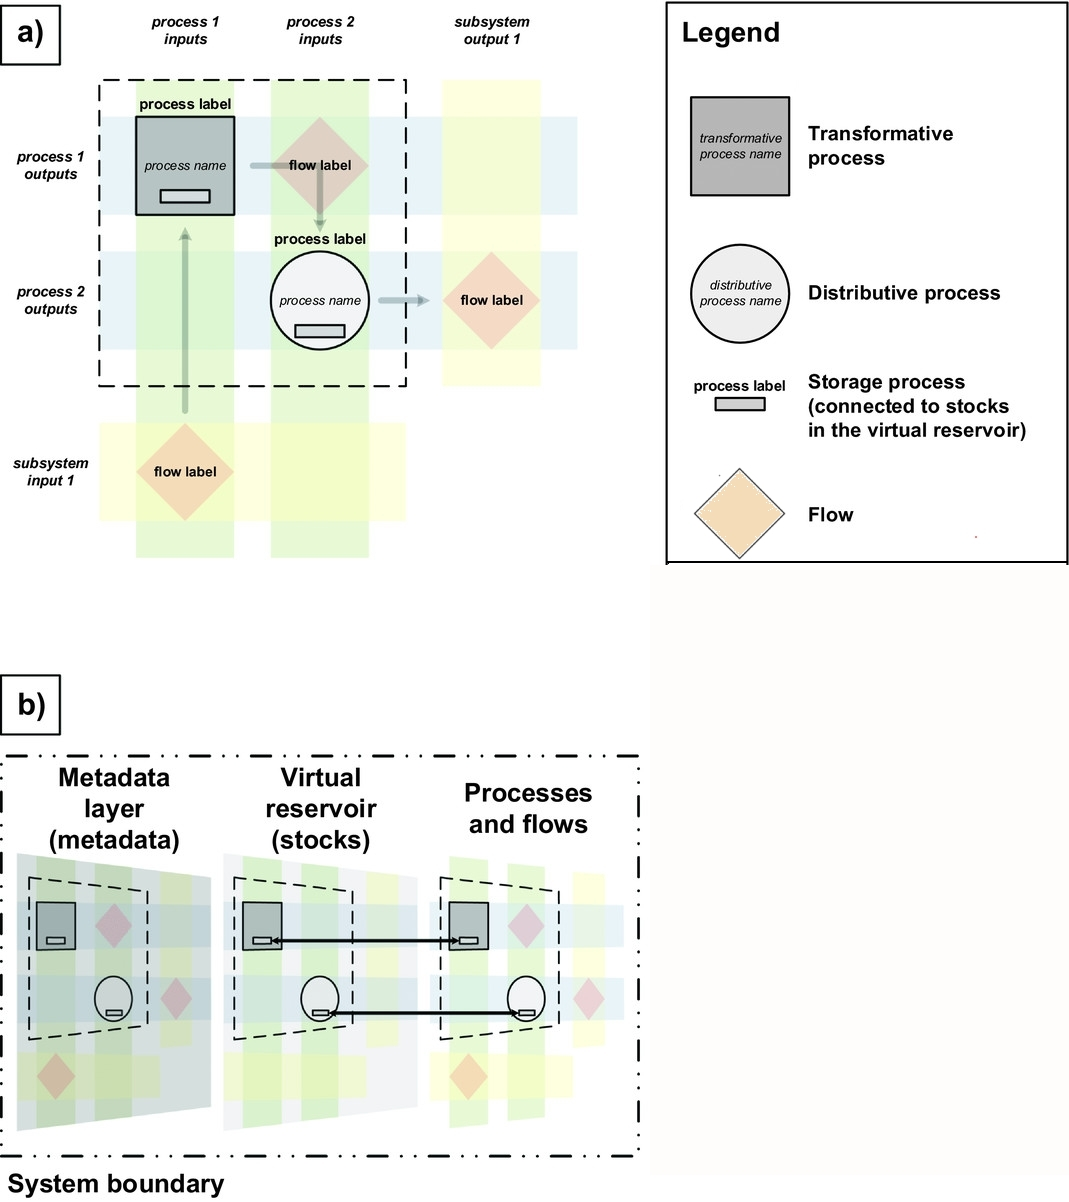
\includegraphics[width=0.6\textwidth]{images/umis_aspects.jpg}
\caption{(a) Key aspects of a UMIS diagram, visualizing it in a matrix style. Contains transformation, distribution and Storage processes as well as 3 flows. The processes lie on the diagonal and the flows are on the row of the origin process and the column of the destination process (b) The orientation of the virtual reservoir and metadata layer in reference to processes and flows. Flows depicted by grey arrows in (a) and conceptual linkages denoted by black arrows in (b) are for illustration and are not properties of UMIS diagrams. UMIS = Unified Materials Information System. Adapted from \cite{myers2019unified}}
\label{fig:umis_aspects}
\end{figure}

\subsubsection{Mass Balancing}
MFA, IOA and LCA all share core modelling concepts. Each methodology involve a separation background and foreground systems, with the background system acting as a more generic supplier of inputs and outputs to the more detailed foreground system \cite{pauliuk2016prospective}. The foreground system is often modelled through a system of equations and constraints, but one common concept to all methodologies is that of mass balancing. The idea of this is that throughout the entire system, matter must be conserved. Therefore the total mass of a given material entering a process must be equal to the total mass leaving \cite{brunner2004practical}. This is defined by the following equation:

Where $i,j \in \{1,..,n\} $ are the processes in the system, $f_{ij}$ is a flow from process $i$ to $j$, $q_i$ and $o_i$ are the inflow and outflow between process $i$ and the background system respectively, and $s_i$ is the stock being supplied to or coming from storage:     

\begin{equation}
    \forall i, q_i + \sum^{n}_{j}f_{ji} = \sum^{n}_{j}f_{ij} + o_{i} \pm{s_i} 
\end{equation}

Further constraints can be supplied in the form of transfer coefficients which allocate the total amount of material flowing into the process amongst the flows leaving the process. With $a_{ij}$ being the transfer coefficient of the flow from process $i$ to $j$, $s_i$ is stock coming from storage (which may be 0) and $z_i$ as the total of all inflows to process $i$, this can be defined as:

\begin{equation}
    z_i = q_i + \sum^{n}_{j}f_{ji} + s_i
\end{equation}



\begin{equation}
    f_{ij} = z_{i}a_{ij}
\end{equation}

% TODO Fix this up
Whilst Myers et al. have demonstrated how material systems in LCA, MFA, IOA studies can be visualized as UMIS diagrams \cite{myers2019unified}, no work has be done to use UMIS structured data in a computational model. In order to demonstrate UMIS's suitability as a structuring system for data in a computational model I will develop a calculation engine for propagating uncertainty through UMIS structured systems.

\section{Uncertainty in IE}
\subsection{What is uncertainty?}
Common practice in IE research is to first define the system in terms of stocks, flows and processes and then identify values for the quantities of stock and flow. These observed values have an associated uncertainty which leads to an uncertainty in model outputs. As IE studies can be used to guide economic and political decisions, it is important to incorporate uncertainty into the results. A study by Danius and Burstr\"om \cite{danius2001regional} found that initial conclusions drawn when studying the flow of nitrogen were inconclusive when data uncertainties were taken into account. Therefore in cases where a comparison of systems are being conducted, the uncertainty around both systems must be taken into account to ensure that the results found are significant and cannot be attributed to variation in underlying data. As such, uncertainty is an important and well studied topic in the fields of LCA, IOA and MFA \cite{temursho201712, laner2014systematic, heijungs2004review}.

The sources of uncertainty can be separated into two kinds \cite{ferson1996different}. The first is aleatory uncertainty which comes from randomness in the underlying value. This is where either the method of measuring the value has an uncertainty around it so the precise value is unknown, or the value itself is non-deterministic. The second kind is epistemic which refers to generalizations about the value. One cause can originate from when values vary over space and time, therefore the value for a time period (e.g one year) or a geographic area (e.g the entire UK) can have an associated uncertainty. Another source can be subjective judgement such as when an unknown value is estimated based on a known value. Other causes can include scientific disagreement over the true value of a quantity, imprecise language on what the quantity refers to (e.g a material being said to be mostly carbon), and approximation in parameters in order to describe the system as a mathematical model. Epistemic uncertainty is potentially reducible through further investigation, however due to feasibility constraints it is sometimes unavoidable \cite{laner2014systematic}.

Further forms of epistemic uncertainty can be caused by possibilities in how the system is defined or described, however as we are looking at a general algorithm for propagating uncertainty in systems, this can be seen as out of scope. Instead, I will focus on uncertainty in specific parameter values.

\subsection{Incorporating Uncertainty into UMIS}
In \cite{laner2014systematic}, Laner et al. describe a five step procedure for incorporating uncertainty into MFA studies. These can be found in figure \ref{fig:incorp uncertainty procedure}:

\begin{figure}[h!]
    \begin{enumerate}
        \item Establish mathematical model
        \begin{itemize}
            \item Define system elements and relationships between the elements
            \item Define equations based on mass balance principle
        \end{itemize}
        
        \item Characterize data uncertainty
        \begin{itemize}
            \item Evaluate information about data (model parameters, inputs and outputs)
            \item Define characterizing functions for uncertainty
        \end{itemize}
        
        \item Combine data and mathematical model
        \begin{itemize}
            \item Balance model and cross-check data
            \item Evaluate plausibility and reconcile data (iterative)
            \item Produce a calibrated model using all available data
        \end{itemize}
        
        \item Calculate uncertainty for calibrated model
        \begin{itemize}
            \item Propagate uncertainty through the model and calculate uncertainty of stocks and flows
            \item Interpret uncertainty estimates for resultant values from model 
        \end{itemize}
        
        \item Analyze sensitivity \& develop scenarios
        \begin{itemize}
            \item Identify critical model parameters
            \item Change parameters to perform scenario analysis
        \end{itemize}
    \end{enumerate}
    \caption{Source: \cite{laner2014systematic}}
    \label{fig:incorp uncertainty procedure}
\end{figure}

% IF you need to pad stuff out you can put another paragraph here about other ways they characterize uncertainty

UMIS provides a method for structuring stocks and flows data into the system described in step one of this procedure however does not explicitly specify a unified way for specifying how the uncertainty around data values must be described. Current development on STAFDB and in the Metabolism of Cities project favours an approach investigated by Laner in \cite{laner2016novel}. This strategy combines the use of a pedigree matrix to classify data quality, as defined by Weidema and Wesnaes \cite{weidema1996data}, and the application of data quality to uncertainty by Hedbrandt and S\"orme \cite{hedbrant2001data}. The pedigree matrix provides five criteria of data quality (reliability, completeness, temporal correlation and geographical correlation). When a data point is recorded it is given a score for each criteria. The score is combined with a sensitivity level to provide a coefficient of variation. The data point can then be modelled as a normally distributed random variable with a standard deviation related to its coefficient of variation. As stocks and flow values can never be negative and can have asymmetrical properties, it can be appropriate to model the data point as a log-normal random variable. Therefore Laner also provides a method for characterizing data quality as an uncertainty factor which relates to the standard deviation of a log-normal distribution. Therefore Laner's work could be used to convert descriptions of a data point's uncertainty from quality scores to probability density functions.

Whilst the above approach provides a method for characterizing the uncertainty of individual data points independently, it does not provide support for combining the the data points as a system. This is key to steps 3 and 4 of the procedure in figure \ref{fig:incorp uncertainty procedure}. To do this the data must be arranged as a mathematical model and the uncertainties of each model parameter must be calculated in respect to each other. Furthermore, a framework must be developed to infer uncertainty estimates for values calculated by the model. In \cite{lupton2018incremental}, Lupton et al. apply a Bayesian inference approach for propagating uncertainty through a model of plastic flows in Austria in 2005. In this paper, Lupton characterizes uncertainty of model parameters as normal distributions. I expand on this approach by generalising it to UMIS specified data and allowing for model parameters to be specified using log-normal distributions also.

\section{Aims}
Below are the aims for this dissertation:

\begin{enumerate}
    \item Investigate literature in propagating uncertainty through industrial ecology models
    \item Develop a program to create a model from UMIS formatted data and propagate uncertainty through it
    \item Add support for representing uncertainty through normal, log-normal and uniform distributions
    \item Evaluate the accuracy and performance of the program
\end{enumerate}
\begin{comment}

Uncertainty
    - Why is it important to show uncertainty?
        - 
    - What are the methods for showing uncertainty?
    - Why is it important to hav a flexible method for showing uncertainty?
    - Need to show uncertainty
        - All studies are used to inform decision making
        - As such uncertainty has been the subject of various literature reviews in the fields of IOA, MFA and LCA, cite cite cite
        - Impairs reliability
        - Important when considering results
        - Can determine if results are significant compared to uncertainty
        - Environmental impacts and indicators are often calculated directly from    values, need to have accurate uncertainty around those values in order to   confidently talk about environmental impact
    - Sources of uncertainty
        Because IE studies often work on an average (i.e average amount of copper, average amount of zinc flowing through)
        
        read this one, take notes, read the lca one quickly, take notes, see how IOA one is important
    - Methods of dealing with and calculating uncertainty
        - Talk about 2 things that aren't related to probabilistic
        - Talk about the Fuzzy set theory, sensitivity analysis, stan, probabilistic and then lupton and then say where mine fits in 
    - Reliability scores (talk in regards to STAFDB and UMIS, ecoinvent scores)
        - Useful when integrating data from across studies
        - Need for lognormal
        - Need to ensure that consistency is kept according to the later laner paper
  
 - Transformation processes have only one outflow
 - Visualized here as a matrix
- Metabolism of Cities
    - Digital research lab created by Paul Hoekman designed to store and facilitate Industrial Ecology research.
    - Contains a store of publications, IE data and an online material flow analysis tool that is designed to allow users to easily conduct MFA studies and interface with an online database.
    - Its primary aim is to encourage and allow collaboration between researches to fully undertand the metabolism of resources and energy surrounding specific regions.
    - Current
- Industrial Ecology
    What is it
    What methods does it use
        LCA
        IOA
        MFA
- STAFDB
   - over the past 20 years the graedal research group at yale university have compiled Industrial Ecological data covering over 60 chemical elements and over 100,000 data entries
   - The data from this has been extracted and placed into YSTAFDB, currently work is continuing to develop STAFDB, a community driven database that enhances YSTAFDB by making it more user friendly and dealing with problems related to divergent disaggregation.
   Disaggregation is where a classification of data is separated into its constituent parts. For example data about cars could be separated into electric or non-electric vehicles as well as large cars or small cars. If two studies were to disaggregate data in different ways, data about the same objects may be counted twice when structured into the same system 
   -UMIS provides a way for structuring YSTAFDB data in a methodology agnostic manner, by enforcing the data to be structured in a directed bipartite graph as well as including a separator flag for processes and materials to ensure that divergent disaggregation is detected.
   - 2 dimensions of edges, one for the tree another for the system (graph)
   - Matrix and layers
- UMIS
 - Ontology
 - What UMIS does
 - Vocabulary based on MFA
 - Allows for dissagregation
 - Difference between communication diagrams and UMIS
 - Each study can still have its own communication diagrams
 - The data can also be represented in a UMIS diagram and stored in a common DB
 - This allows data to be shared between studies
 - Nulius in verba: Can store data online for transparancy
 - Components of a umis diagram (basically only need to say its a directed bipartite graph
 - Talk about MFA terminology
  - Talk about stafdb
 - You're focusing on how this thing is relevant
 -  
- Metabolism of Cities
- Uncertainty
    - Uncertainty scores
    - Ecoinvent
    - Need to be able to flexibly support different forms of uncertainty
   
- No work as of yet has been done to use UMIS as a feed in for a computational model
-   
    
- Show how data referenced in UMIS can be referenced in databases and computational models
    - 
- What is the project topic or problem being investigated?
- Why is the topic important, why should the reader care about it?
- What are the central challenges involved and why are they significant?
\end{comment}



% -----------------------------------------------------------------------------

\chapter{Technical Background}
\label{chap:technical}

{\bf A compulsory chapter,     of roughly $10$ pages} 
\vspace{1cm} 

\noindent

\begin{comment}
 - The Bipartite directed graph https://onlinelibrary.wiley.com/doi/full/10.1111/jiec.12306
 - Pymc3
  - Lupton
  - Cencic/Stan
  - Cencic offer simplex algorithms as a way for automatically constructing the model but do not implement a program to do so
  - Bayesian Inference
  - A fuzzy set-based approach to data reconciliation in material flow modeling,
        - Can talk about this, can suggest that using probability distributions is better because fuzzy sets have trapezoidal and triangular membership functions which can be modelled as distributions if you use pymc3 correctly
  - we want a genral approach to specifying the outputs of the model
  - For execution, a low level of sample acceptance is indicative of a mistake when describing the system, therefore the system must be re-described
  - Execution, umis as classes (decisions)
  - Evaluation - turn graedal diagram into UMIS diagram
  - Evaluation - Lognormal, does that work
  
  - So its good that you've studied this stuff because you'll want to talk about it in the technical thing
  - First read other technical things and see if they are similar
  - I think for the technical thing the topics are
    - AISHA, read that to see if they indicated a good way to explain the ways that   they built the constraints automatically
    - Fuzzy set theory method 
    - STAN method
    - Mathematical MFA method
    - Sensitivity analysis method
    - Probabilistic MFA, what I use
    - Monte Carlo Markov Chains
    - No-U-Turn, metropolis hastings
    - Pymc3
    
\end{comment}
This chapter is intended to describe the technical basis on which execution
of the project depends.  The goal is to provide a detailed explanation of
the specific problem at hand, and existing work that is relevant (e.g., an
existing algorithm that you use, alternative solutions proposed, supporting
technologies).  

Per the same advice in the handbook, note there is a subtly difference from
this and a full-blown literature review (or survey).  The latter might try
to capture and organise (e.g., categorise somehow) {\em all} related work,
potentially offering meta-analysis, whereas here the goal is simple to
ensure the dissertation is self-contained.  Put another way, after reading 
this chapter a non-expert reader should have obtained enough background to 
understand what {\em you} have done (by reading subsequent sections), then 
accurately assess your work.  You might view an additional goal as giving 
the reader confidence that you are able to absorb, understand and clearly 
communicate highly technical material.

% -----------------------------------------------------------------------------

\chapter{Project Execution}
\label{chap:execution}

{\bf A topic-specific chapter, of roughly $15$ pages} 
\vspace{1cm} 

\noindent
This chapter is intended to describe what you did: the goal is to explain
the main activity or activities, of any type, which constituted your work 
during the project.  The content is highly topic-specific, but for many 
projects it will make sense to split the chapter into two sections: one 
will discuss the design of something (e.g., some hardware or software, or 
an algorithm, or experiment), including any rationale or decisions made, 
and the other will discuss how this design was realised via some form of 
implementation.  

\noindent
Note that it is common to include evidence of ``best practice'' project 
management (e.g., use of version control, choice of programming language 
and so on).  Rather than simply a rote list, make sure any such content 
is useful and/or informative in some way: for example, if there was a 
decision to be made then explain the trade-offs and implications 
involved.


% -----------------------------------------------------------------------------

\chapter{Critical Evaluation}
\label{chap:evaluation}

{\bf A topic-specific chapter, of roughly $15$ pages} 
\vspace{1cm} 

\noindent
This chapter is intended to evaluate what you did.  The content is highly 
topic-specific, but for many projects will have flavours of the following:

\begin{enumerate}
\item functional  testing, including analysis and explanation of failure 
      cases,
\item behavioural testing, often including analysis of any results that 
      draw some form of conclusion wrt. the aims and objectives,
      and
\item evaluation of options and decisions within the project, and/or a
      comparison with alternatives.
\end{enumerate}

\noindent
This chapter often acts to differentiate project quality: even if the work
completed is of a high technical quality, critical yet objective evaluation 
and comparison of the outcomes is crucial.  In essence, the reader wants to
learn something, so the worst examples amount to simple statements of fact 
(e.g., ``graph X shows the result is Y''); the best examples are analytical 
and exploratory (e.g., ``graph X shows the result is Y, which means Z; this 
contradicts [1], which may be because I use a different assumption'').  As 
such, both positive {\em and} negative outcomes are valid {\em if} presented 
in a suitable manner.

% -----------------------------------------------------------------------------

\chapter{Conclusion}
\label{chap:conclusion}

{\bf A compulsory chapter,     of roughly $5$ pages} 
\vspace{1cm} 

\noindent
The concluding chapter of a dissertation is often underutilised because it 
is too often left too close to the deadline: it is important to allocation
enough attention.  Ideally, the chapter will consist of three parts:

\begin{enumerate}
\item (Re)summarise the main contributions and achievements, in essence
      summing up the content.
\item Clearly state the current project status (e.g., ``X is working, Y 
      is not'') and evaluate what has been achieved with respect to the 
      initial aims and objectives (e.g., ``I completed aim X outlined 
      previously, the evidence for this is within Chapter Y'').  There 
      is no problem including aims which were not completed, but it is 
      important to evaluate and/or justify why this is the case.
\item Outline any open problems or future plans.  Rather than treat this
      only as an exercise in what you {\em could} have done given more 
      time, try to focus on any unexplored options or interesting outcomes
      (e.g., ``my experiment for X gave counter-intuitive results, this 
      could be because Y and would form an interesting area for further 
      study'' or ``users found feature Z of my software difficult to use,
      which is obvious in hindsight but not during at design stage; to 
      resolve this, I could clearly apply the technique of Smith [7]'').
\end{enumerate}

% =============================================================================

% Finally, after the main matter, the back matter is specified.  This is
% typically populated with just the bibliography.  LaTeX deals with these
% in one of two ways, namely
%
% - inline, which roughly means the author specifies entries using the 
%   \bibitem macro and typesets them manually, or
% - using BiBTeX, which means entries are contained in a separate file
%   (which is essentially a databased) then inported; this is the 
%   approach used below, with the databased being dissertation.bib.
%
% Either way, the each entry has a key (or identifier) which can be used
% in the main matter to cite it, e.g., \cite{X}, \cite[Chapter 2}{Y}.

\backmatter

\bibliography{dissertation}

% -----------------------------------------------------------------------------

% The dissertation concludes with a set of (optional) appendicies; these are 
% the same as chapters in a sense, but once signaled as being appendicies via
% the associated macro, LaTeX manages them appropriatly.

\appendix

\chapter{An Example Appendix}
\label{appx:example}

Content which is not central to, but may enhance the dissertation can be 
included in one or more appendices; examples include, but are not limited
to

\begin{itemize}
\item lengthy mathematical proofs, numerical or graphical results which 
      are summarised in the main body,
\item sample or example calculations, 
      and
\item results of user studies or questionnaires.
\end{itemize}

\noindent
Note that in line with most research conferences, the marking panel is not
obliged to read such appendices.

% =============================================================================

\end{document}
